\begin{post}
	\postdata{It's raining in paradise}{2011}{10}{15}{22}{48}{26}
	\begin{content}
\textit{``Thunder and lightning, not so frightening, anymore...''}

After several nice days the hell has broken loose in here. The rain was so heavy that only going from the dorm to the SUPEX building made me \sout{wet} completely soaked. I have a feeling that it might have something to do with my non-existent umbrella, but that's just me. Me and Marc were planning to go to Lotte Dept. Store, because he needed some clothes and I need some shoes, since my beloved Nike's gave up and fell apart. Since we are no wusses, we decided to walk to the subway station, despite the thunderstorm and rain, so I only had to stop at 7eleven to buy an umbrella (a lovely umbrella, branded ``Pierre Balmain — Paris'', for 9000KRW), to be able to make it to Hoegi station without melting (because I am such a sweet guy). Since the subway was completely packed, you can imagine the ``atmosphere'' there, created by wet people and umbrellas. Fortunately, the other train from Wangsimni was less crowded and better ventilated.

Anyhow, there is no point in describing our shopping. I can only say that Marc bought his stuff, while I did not find any nice shoes (except for one Fred Perry sneakers, which were however a little too expensive — I keep them as a last resort backup). The best part of the trip was however the visit to the shooting range. At the Lotte complex at Jamsil station, there is, apart from Lotte World, Lotte Hotel, Lotte Dept. Store, Lotte Cinema and Lotte Mart (damn, there is a whole lotta Lotte!) a small indoor shooting range. Both me and Marc tried the world famous Glock 17, a rather small 9mm semi-automatic gun.

\begin{figure}[h]
\centering
\fbox{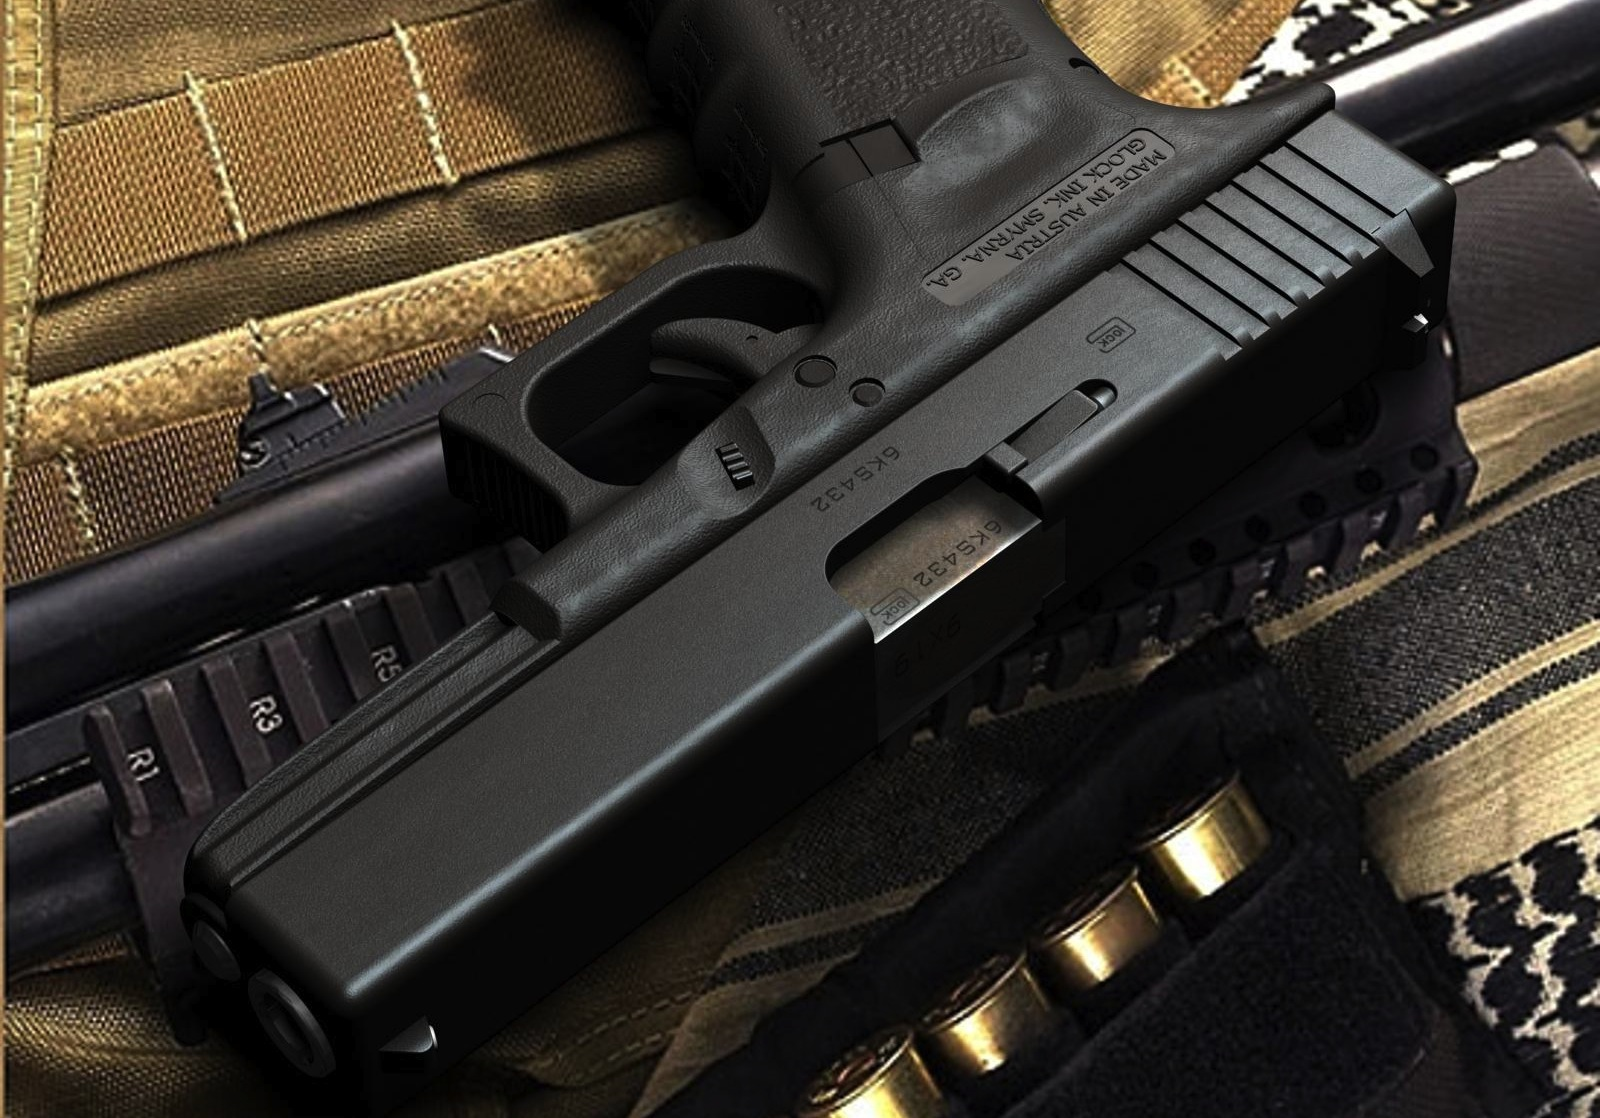
\includegraphics[width=0.5\textwidth]{photos/10/15/glock.jpg}}
\caption{Glock 17}
\end{figure}

We each fired 10 rounds, Marc scored 97, I did only 91, but it was not about the number. The mere feeling of holding the gun is so awesome and frightening at the same time. When you fire, you just need so little force to unleash a force so much bigger and powerful. I definitely want to repeat this some day, preferably more rounds, but I think I don't want to own a gun. Ever

On a completely different note, we have decided to go to Tokyo after exams, so ``YAY!''. On top of that, sunny times are supposedly over, since the have already turned on the heating in the dorms. Bye-bye aircon, sundresses and shorts. Hello heaters, coats and long pants.
	\end{content}
\end{post}
